\section{Timing}\label{sec:timing}
\sectionstate{open}{PLAN\_42 (\texttt{42\_time\_resolution.py}) -- hits-based; waveform port is D3}
\intent{The time resolution of a chamber against the scintillator trigger, which fixes how well the absolute drift
depth (and so the $z$ of a track) is known.}

\tbw{Method: scintillator-trigger reference, DREAM fine timestamp. The hits value (33\,ns) is not quoted; waveform result to come.}
\analysis{D3}{time resolution on waveforms}
\begin{figure}[t]
  \centering
  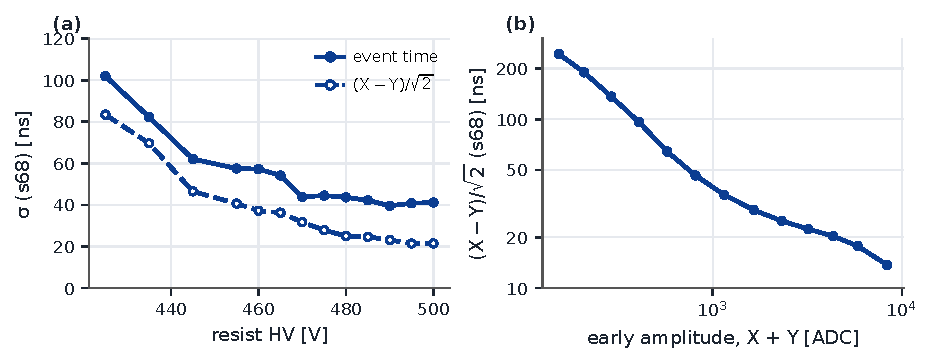
\includegraphics[width=0.95\linewidth]{timing}
  \caption{\tbw{Time resolution of M3-matched cosmic tracks on the bench: (a) against the resist HV in the scans, the event time and the uncorrelated part $(t_X-t_Y)/\sqrt2$; (b) the uncorrelated part against the signal size, with det4 at SPS (open grey); (c) on the golden rows, the event time against the trigger, the part common to X and Y, and the uncorrelated part. The trigger term is 42\,ns.}}
  \label{fig:timing}
\end{figure}
